


\newcommand{\suppresultsfigwidth}{1.14in}
\newcommand{\suppresultscropwidth}{0.69in}

\newcommand{\cropgreek}[1]{
  \makecell{
  \includegraphics[trim={202px 201px 202px 203px}, clip, width=\suppresultscropwidth]{#1} \\
  \includegraphics[trim={221px 132px 199px 288px}, clip, width=\suppresultscropwidth]{#1}
  }
}


\newcommand{\cropcube}[1]{
  \makecell{
  \includegraphics[trim={300px 309px 136px 127px}, clip, width=\suppresultscropwidth]{#1} \\
  \includegraphics[trim={120px 132px 316px 304px}, clip, width=\suppresultscropwidth]{#1} 
  }
}



\begin{figure}[t]
\centering
\scriptsize
\begin{tabular}{@{}c@{}c@{}c@{}c@{}c@{}c@{}}
\makecell[c]{
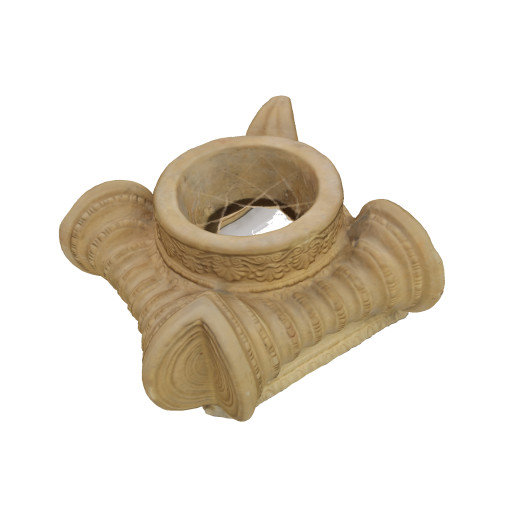
\includegraphics[trim={0px 0px 0px 100px}, clip, width=\suppresultsfigwidth]{figs/dvox_images/gt_greek_575.jpg}
\\
\scenename{Pedestal}
}
&
\cropgreek{figs/dvox_images/gt_greek_575.jpg} &
\cropgreek{figs/dvox_images/ours_greek_575.jpg} &
\cropgreek{figs/dvox_images/llff_greek_575.jpg} &
\cropgreek{figs/dvox_images/srn_greek_575.jpg} &
\cropgreek{figs/dvox_images/nv_greek_575.jpg} \\
\makecell[c]{
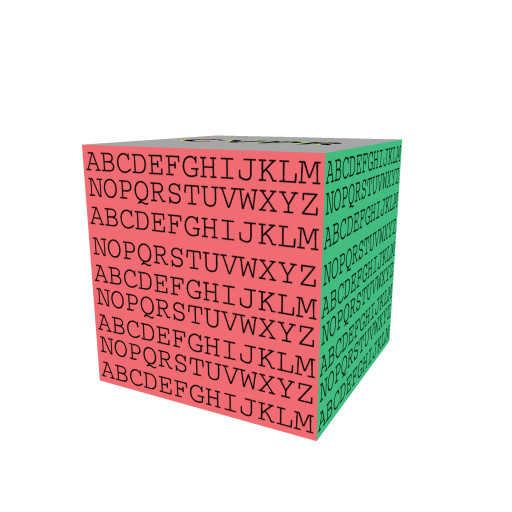
\includegraphics[trim={0px 0px 0px 100px}, clip, width=\suppresultsfigwidth]{figs/dvox_images/gt_cube_160.jpg}
\\
\scenename{Cube}
}
&
\cropcube{figs/dvox_images/gt_cube_160.jpg} &
\cropcube{figs/dvox_images/ours_cube_160.jpg} &
\cropcube{figs/dvox_images/llff_cube_160.jpg} &
\cropcube{figs/dvox_images/srn_cube_160.jpg} &
\cropcube{figs/dvox_images/nv_cube_160.jpg} \\
& Ground Truth & NeRF (ours) & LLFF~\cite{mildenhall19} & SRN~\cite{srn} & NV~\cite{neuralvolumes}
\end{tabular} 
\caption{Comparisons on test-set views for scenes from the DeepVoxels~\cite{deepvoxels} synthetic dataset. The objects in this dataset have simple geometry and perfectly diffuse reflectance. Because of the large number of input images (479 views) and simplicity of the rendered objects, both our method and LLFF~\cite{mildenhall19} perform nearly perfectly on this data. LLFF still occasionally presents artifacts when interpolating between its 3D volumes, as in the top inset for each object. SRN~\cite{srn} and NV~\cite{neuralvolumes} do not have the representational power to render fine details.}
\label{fig:synthresults}
\end{figure}